\documentclass{article}

\usepackage{amsmath}
\usepackage{amsthm}
\usepackage{amsfonts}
\usepackage{listings}
\usepackage{xcolor} 
\usepackage{graphicx}
\usepackage{subcaption}
\usepackage[utf8]{inputenc}
\usepackage[russian]{babel}
\usepackage{float}

\DeclareMathOperator*{\argmax}{arg\,max}
\DeclareMathOperator*{\argmin}{arg\,min}

\DeclareMathOperator{\diag}{diag}
\DeclareMathOperator{\tr}{tr}
\DeclareMathOperator{\vect}{vec}
\DeclareMathOperator{\cone}{cone}
\DeclareMathOperator{\dist}{dist}

\newcommand{\R}{\mathbb{R}}
\newcommand{\RV}[1] {\mathbb{R}^{#1}}
\newcommand{\RM}[2] {\mathbb{R}^{#1 \times #2}}
\newcommand{\norm}[1]{\left\lVert#1\right\rVert}

\title{Домашнее задание II}
\author{Кобылянский А.В. \\ Группа 5381 \\ Вариант 2}
\date {}


\definecolor{mygreen}{RGB}{28,172,0} % color values Red, Green, Blue
\definecolor{mylilas}{RGB}{170,55,241}


\begin{document}

    \lstset{language=Python,
        breaklines=true,
        keywordstyle=\color{blue},
        identifierstyle=\color{black},
        stringstyle=\color{mygreen},
        commentstyle=\color{gray},
        showstringspaces=false,%without this there will be a symbol in the places where there is a space
        numbers=left,%
        numberstyle={\tiny \color{black}},% size of the numbers
        numbersep=9pt, % this defines how far the numbers are from the text
        emph=[1]{for, in, while, break},emphstyle=[1]\color{red}, %some words to emphasise
    }

    \pagenumbering{gobble}
    \maketitle
    \newpage
    \pagenumbering{arabic}
         
    \subsection*{Задача 1}
    
    Пользуясь определением выпуклой функции
    \begin{equation*}
         f(\lambda x + (1 - \lambda)y) \le \lambda f(x) + (1 - \lambda)f(y)
    \end{equation*}
    Где $\lambda \in [0, 1]$, показать, что следующие функции выпуклые
    
    \begin{align*}
         f(x) &= \norm{x}_1, x \in \R^n, (l_1-norm) \\
         f(x) &= \norm{x}_2, x \in \R^n, (l_2-norm) \\
         f(x) &= \norm{x}_{\infty}, x \in \R^n, (infinity-norm) 
    \end{align*}
    
    Если для функции $\norm{.} : \R^n \rightarrow \R$ выполняются 2 аксиомы нормы    
    \begin{align*}
         &1. \forall \alpha \in \R \, \forall x \in \R^n : \norm{\alpha x} = |\alpha|\norm{x}\\
         &2. \forall x, y \in \R^n : \norm{x + y} \le \norm{x} + \norm{y}
    \end{align*}
    то эта функция выпукла
    \begin{align*}
         \norm{\lambda x + (1 - \lambda)y} \le \norm{\lambda x} + \norm{(1 - \lambda)y} = 
         |\lambda| \norm{ x} + |1 - \lambda| \norm{y} = \lambda \norm{ x} + (1 - \lambda) \norm{y} 
    \end{align*}
    
    Выполнение первой аксиомы очевидно для всех трех функций. Покажем, что выполняется вторая аксиома.
    \bigbreak
    
    1. $f(x) = \norm{x}_1 = \sum_{i = 1}^{n} |x_i|$
    
    Так как $\forall a, b \in \R : |a + b| \le |a| + |b|$, то
    \begin{align*}
         \sum_{i = 1}^{n} |x_i + y_i| \le 
         \sum_{i = 1}^{n} |x_i| + |y_i|  = 
         \sum_{i = 1}^{n} |x_i| + \sum_{i = 1}^{n} |y_i|
    \end{align*}
    
    Левая сумма поэлементно меньше правой. Аксиома выполняется.
    \bigbreak
    
    2. $f(x) = \norm{x}_2 = \sqrt{ \sum_{i = 1}^{n} |x_i|^2} = \sqrt{x^Tx}$
    \begin{align*}
         \sqrt{(x + y)^T(x + y)} &\le \sqrt{x^Tx} + \sqrt{y^Ty} \\
         (x + y)^T(x + y) &\le x^Tx + y^Ty + 2\sqrt{x^Txy^Ty} \\
         x^Tx + y^Ty + 2x^Ty &\le x^Tx + y^Ty + 2\sqrt{x^Txy^Ty} \\
         x^Ty &\le \sqrt{x^Txy^Ty} 
    \end{align*}
    
    В первом неравенстве обе части неотрицательны, так что можно возвести их в квадрат, получится эквивалентное неравенство.
    
    Последнее неравенсто - более слабая версия неравенства Коши — Буняковского.
    \begin{align*}
         \forall \lambda \in \R \, \forall x, y \in \R^n : (\lambda x + y)^T(\lambda x + y) \ge 0 \\
         \lambda^2 x^Tx + 2\lambda x^Ty + y^Ty \ge 0 \\
         D = 4(x^Ty)^2 - 4x^Txy^Ty \le 0 \\
         |x^Ty| \le \sqrt{x^Txy^Ty}
    \end{align*}
    \bigbreak
    
    3. $f(x) = \norm{x}_\infty = \max |x_i|$
    \begin{align*}
         \max |x_i + y_i| = |x_m + y_m| \le |x_m| + |y_m| \le \max |x_i| + \max |y_i|
    \end{align*}
    \bigbreak
    
    \subsection*{Задача 2}
    Пусть $S = \{x \in \R^n \mid  x^TAx + b^Tx + c \le 0\}$, где $A$ - симметричная матрица. Показать, что множество $S$ выпукло, если $A \succeq 0$ (матрица $A$ является положительно полуопределенной). 
    \bigbreak
    
    Множество линий уровня выпуклой функции 
    \begin{align*}
         Lev_f (\alpha) := \{ x \mid f(x) \le \alpha \}
    \end{align*}
    является выпуклым.
    
    Покажем, что наша функция выпукла
    \begin{align*}
         f(x) &= x^TAx + b^Tx + c\\
         df(x) &= 2x^TAdx + b^Tdx = (2Ax + b)^Tdx\\
         d( (2Ax + b)^Tdx_1) &= (dx_1)^T2Adx_2\\
         \nabla^2 f &= 2A \succeq 0
    \end{align*}
    По дифференциальному признаку функция выпукла, значит выпукло и исходное множество.
    \bigbreak
    
    \subsection*{Задача 3}
    Пусть $S \subset \R^n$ - замкнутое выпуклое множество и $y \in \R^n$. Введем обозначение $\Pi_s(y)$, обозначающее евклидову проекцию точки $y$ на множество $S$, Можно показать, что для любой точки $x \in S$ выполняется неравенство 
    \begin{align}
         (x - \Pi_s(y))^T(y - \Pi_s(y)) \le 0 \: 
    \end{align}
    
    Доказать, что для любых $z, y \in \R^n$ верно
    \begin{align*}
         \norm{\Pi_s(z) - \Pi_s(y)}_2 \le \norm{z - y}_2 
    \end{align*}
    
    Доказательство
    \begin{align*}
        \norm{(\Pi_s(z) - \Pi_s(y)) - (z - y)}^2 &= 
        \norm{\Pi_s(z) - \Pi_s(y)}^2 + \norm{z - y}^2 - 2(\Pi_s(z) - \Pi_s(y))^T(z - y) \\
        (\Pi_s(z) - \Pi_s(y))^T(z - y) &=
        \norm{\Pi_s(z) - \Pi_s(y)}^2 + (\Pi_s(z) - \Pi_s(y))^T(z - \Pi_s(z)) +\\ 
        &+ (\Pi_s(z) - \Pi_s(y))^T(\Pi_s(y) - y) \\
        \norm{z - y}^2 - \norm{\Pi_s(z) - \Pi_s(y)}^2 &= 
        \norm{(\Pi_s(z) - \Pi_s(y)) - (z - y)}^2 +\\
        &+ 2(\Pi_s(z) - \Pi_s(y))^T(z - \Pi_s(z)) +\\
        &+ 2(\Pi_s(z) - \Pi_s(y))^T(\Pi_s(y) - y) \\
    \end{align*}
    
    В последнем равенстве в правой части первое слагаемое неотрицательно, потому что это квадрат нормы, второе и третье слагаемое неотрицательны из-за неравенства (1). Значит
    \begin{align*}
        \norm{z - y}^2 - \norm{\Pi_s(z) - \Pi_s(y)}^2 \ge 0 \Rightarrow  
        \norm{\Pi_s(z) - \Pi_s(y)} \le \norm{z - y}
    \end{align*}
    что и требовалось доказать.
    \bigbreak
    
    Это значит, что отображение $\Pi_s(y) : y \mapsto \argmin_{x \in S} \norm{x - y}_2^2$ является нерастягивающим. В случае если для некоторого отображения $F$ выполняется 
    \begin{align*}
        \norm{F(z) - F(y)}_2 < \norm{z - y}_2
    \end{align*}
    то оно называется сжимающим. 
    
    Показать, что композиция нерпстягивающего и сжимающего отображений является сжимающим отображением.
    
    Пусть $F$ - нерастягивающиее отображение, а $G$ - сжимающиее, тогда
    \begin{align*}
        \norm{F(G(z)) - F(G(y))}_2 &\le \norm{G(z) - G(y)}_2 < \norm{z - y}_2\\
        \norm{G(F(z)) - G(F(y))}_2 &< \norm{F(z) - F(y)}_2 \le \norm{z - y}_2
    \end{align*}
    $F \circ G$ и $G \circ F$ являются сжимающими отображениями.
    \bigbreak
    
    \subsection*{Задача 4}
    Рассмотрим задачу оптимизации
    \begin{align*}
        \min_x \norm{x}\\
        s.t. Ax = b
    \end{align*}
    Показать, что $x_*$ является единственным решением этой задачи только если
    \begin{align*}
        T_C(x_*) \cap null(A) = \{0\}
    \end{align*}
    где $C$ - произвольный шар нормы $\norm{.}$, а $null(A) = \{x \mid Ax = 0\}$ обозначает ядро или нуль-пространство линейного оператора $A$.
    \bigbreak
    
    Пусть $T_C(x_*) \cap null(A) \ne \{0\}$
    \begin{align*}
        z - x_* &\in T_C(x_*) \cap null(A) \setminus \{0\} =\\
        &= \cone \{z - x_* \mid \norm{z} \le \norm{x_*} \} \cap \{ x \mid Ax = 0 \} \setminus \{0\} 
    \end{align*}
    тогда 
    \begin{align*}
        z - x_* \ne 0 &\Rightarrow z \ne x_*\\
        z - x_* \in \cone \{z - x_* \mid \norm{z} \le \norm{x_*} \} &\Rightarrow \norm{z} \le \norm{x_*}\\
        z - x_* \in \{ x \mid Ax = 0 \} &\Rightarrow Az = A(z - x_* + x_*) = A(z - x_*) + Ax_* = b 
    \end{align*}
    Значит $x_*$ не единственный минимальный элемент, удовлетворяющий условиям $Ax = b$. 
    \bigbreak
    
    \subsection*{Задача 5}
    Рассмотрим задачи поиска евклидова расстояния между замкнутыми выпуклыми множествами. В общем виде такие задачи можно сформулировать следующим образом:
    \begin{align*}
        \min_{x, y} \norm{x - y}^2\\
        s.t. \: x \in C_1, y \in C_2
    \end{align*}
    
    Пусть $\mathcal{A}$ - центрально симметричный ($a \in \mathcal{A} \Leftrightarrow -a \in \mathcal{A}$) набор векторов ("атомов"), такой, что элементы $\mathcal{A}$ есть крайние точки выпуклой оболочки $\mathcal{A}$, обозначаемой $conv(\mathcal{A})$. Определим атомарную норму для множества $\mathcal{A}$ следующим образом
    \begin{align*}
        \norm{x}_{\mathcal{A}} = \inf \{ t > 0 \mid x \in t conv(\mathcal{A}) \}
    \end{align*}
    
    Пусть $\mathcal{A} = \{(1, 0), (0, 1), (-1, 1), (-1, 0), (0, -1), (1, -1) \}$, $\Phi = [1, 2]$ и $y = 10$. Найти решение задачи.
    \bigbreak
    
    Пусть $\dist(t)$ - расстояние от шара нормы $\norm{.}_{\mathcal{A}}$ с радиусом $t$ до множества $\{x \mid Ax = y\}$. Будем искать 
    \begin{align*}
        t_0 = \min_{  \dist(t) = 0 }{t}    
    \end{align*}
    
    $t_0$ можно найти бинарным поиском, $\dist(t)$ при этом можно вычислить, решая задачу квадратичного программирования. 
    
    Вектор переменных равен $[a, b]$, где $a$ - точка из шара, $b$ точка из $\{x \mid Ax = y\}$. Условия на попадания точки в шар линейны:
    \begin{align*}
          \begin{cases} 
            a_0 + a_1 &\le t\\
            a_0 + a_1 &\ge -t\\
            a_0 &\le t\\
            a_0 &\ge -t\\
            a_1 &\le t\\
            a_1 &\ge -t
        \end{cases}\\
    \end{align*}
    
    Целевую функцию можно записать как
    \begin{align*}
        (a - b)^T(a - b) = [\begin{matrix} a & b\end{matrix}]
            \left[
            \begin{matrix}
                I_2,  & -I_2\\
                -I_2, &  I_2
            \end{matrix}
            \right] 
            \left[
            \begin{matrix}
                a\\
                b
            \end{matrix}
            \right] 
    \end{align*}
    
    \newpage
    Код решения:
    \lstinputlisting[firstline=4, lastline=58]{Source/task5.py}
    
    Визуализация:
    \begin{figure}[ht]
        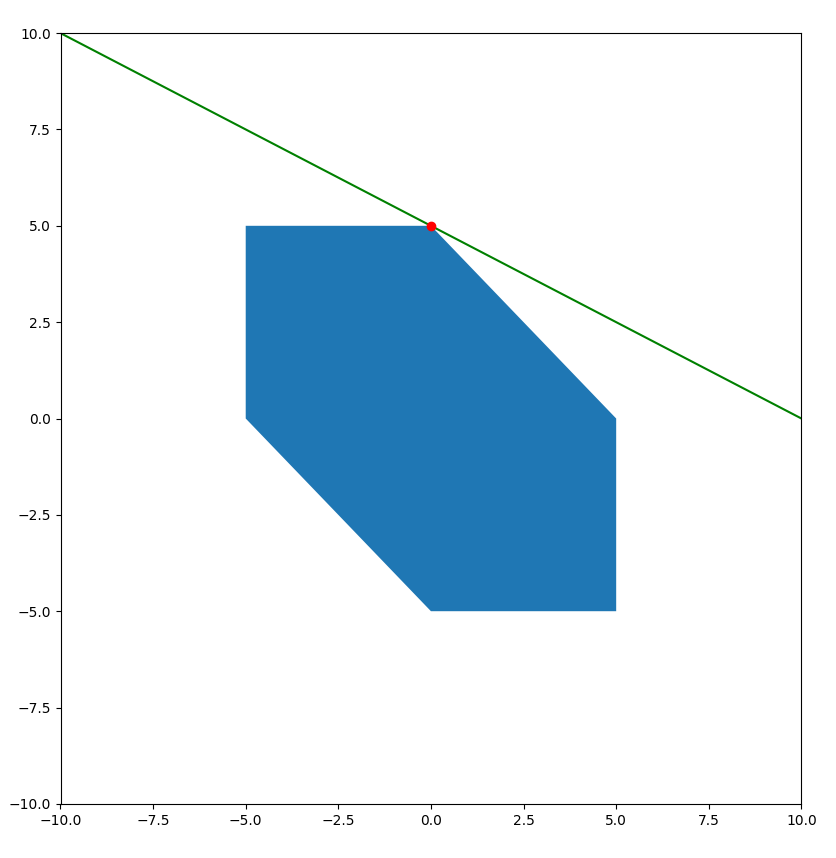
\includegraphics[width=0.8\linewidth]{Screenshots/task5.png}
    \end{figure} 
    
    \newpage
    
    \subsection*{Задача 6}
    Найти значение максимального потока из S в T для графа на рисунке ниже.
    \begin{figure}[h!]
        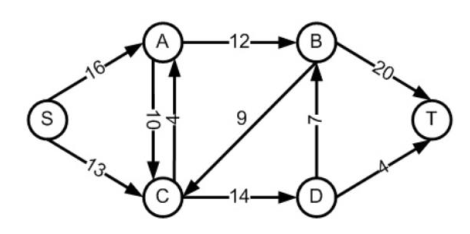
\includegraphics[width=0.8\linewidth]{Screenshots/graph6.png}
    \end{figure}
    Каждое ребро имеет максимальную пропускную способность.
    
    \bigbreak
    Задача линейного программирования:
    \begin{align*}
        \min_x c^Tx\\
        s.t. Gx \le h\\
        Ax = b
    \end{align*}
    Опишем $x, c, G, h, A, b$.
    
    $x$ - вектор потоков через каждое ребро.
    \begin{align*}
        x = [SA, SC, AC, CA, AB, CD, BC, DB, BT, DT]^T
    \end{align*}
    Нам надо максимизировать поток через ребра $BT$ и $DT$ или минимизировать $-(BT + DT)$.
    \begin{align*}
        c = [0, 0, 0, 0, 0, 0, 0, 0, -1, -1]^T
    \end{align*}
    Потоки должны быть неотрицательны и меньше пропускной способности данного ребра.
    \begin{align*}
        G = \left[
            \begin{matrix}
                -I\\
                 I
            \end{matrix}
            \right], 
        h = \left[
            \begin{matrix}
                0\\
                h_1
            \end{matrix}
            \right]
    \end{align*}
    Где $I \in \RM{10}{10}$ - единичная матрица, $0 \in \R^{10}$ - столбец из нулей, $h_1$ - вектор пропускных способностей ребер.
    \begin{align*}
        h_1 = [16, 13, 10, 4, 12, 14, 9, 7, 20, 4]^T   
    \end{align*}
    Для узлов $A, B, C, D$ входящий поток должен быть равен выходящиему.
    \begin{align*}
        &\begin{cases} 
            SA + CA &= AC + AB\\
            AB + DB &= BC + BT\\
            AC + SC + BC &= CA + CD\\
            CD &= DB + DT    
        \end{cases}\\
        &A = \left(
            \begin{matrix}
                1 & 0 & -1 & 1 & -1 & 0 & 0 & 0 & 0 & 0\\
                0 & 0 & 0 & 0 & 1 & 0 & -1 & 1 & -1 & 0\\
                0 & 1 & 1 & -1 & 0 & -1 & 1 & 0 & 0 & 0\\
                0 & 0 & 0 & 0 & 0 & 1 & 0 & -1 & 0 & -1
            \end{matrix}
            \right), \: 
        b = \left(
            \begin{matrix}
                0\\
                0\\
                0\\
                0
            \end{matrix}
            \right)  
    \end{align*}
    
    Код решения
    \lstinputlisting{Source/task6.py}
    
    Найденое решение действительно оптимально. В узел B не может попасть больше чем 19 единиц потока, из D максимум выходит только 4 единицы, $4 + 19 = 23$.
    \bigbreak
    
    \subsection*{Задача 7}
    
    Для заданных постоянных $\Phi \in \RM{m}{n}, y \in \R^m$ и вектора переменных $x \in \R^n$ переформулировать следующие задачи оптимизации как задачи линейного программирования:
    \begin{align*}
        \min_x c^Tx\\
        s.t. Gx \le h\\
        Ax = b
    \end{align*}
    Иными словами, выразить $c, G, h, A, b$ через $\Phi$ и $y$ так, чтобы получились задачи оптимизации, эквивалентные следующим:
    \bigbreak
    
    3. $\min_x \norm{\Phi x - y}_1 \: s.t. \norm{x}_{\infty} \le \gamma$
    
    Пусть $z = \Phi x - y$, $s = [|z_1|, |z_2|, ..., |z_m|]^T$, $\gamma_v$ - вектор со значениями $\gamma$. Вектор переменных установим равным $[s; x]$. Тогда задачу оптимизации можно переписать как
    \begin{align*}
        \min 1^Ts\\
        s.t. \: \Phi x - y &\le s\\
        \Phi x - y &\ge -s\\
        x &\le \gamma_v \\
        -x &\le \gamma_v
    \end{align*}
    Выразми $c, A, b$:
    \begin{align*}
        c = \left[\begin{matrix} 1_v\\ 0_v \end{matrix} \right], \:
        A = \left[
            \begin{matrix}
                -I & \Phi \\
                -I & -\Phi \\
                0_m & I \\
                0_m & -I
            \end{matrix}
            \right], \:
        b = \left[
            \begin{matrix}
                y \\
                -y \\
                \gamma_v\\
                \gamma_v
            \end{matrix}
            \right]
    \end{align*}
    где $0_v, 1_v$ - векторы из нулей и единиц соответственно, $0_m$ - матрица из нулей, $I$ - единичная матрица.
    
    \newpage
    Код решения:
    \lstinputlisting{Source/task7_3.py}
    
    \newpage
    Визуализация решения. Красная точка - $\Phi x_*$, синяя - $y$.
    \begin{figure}[H]
        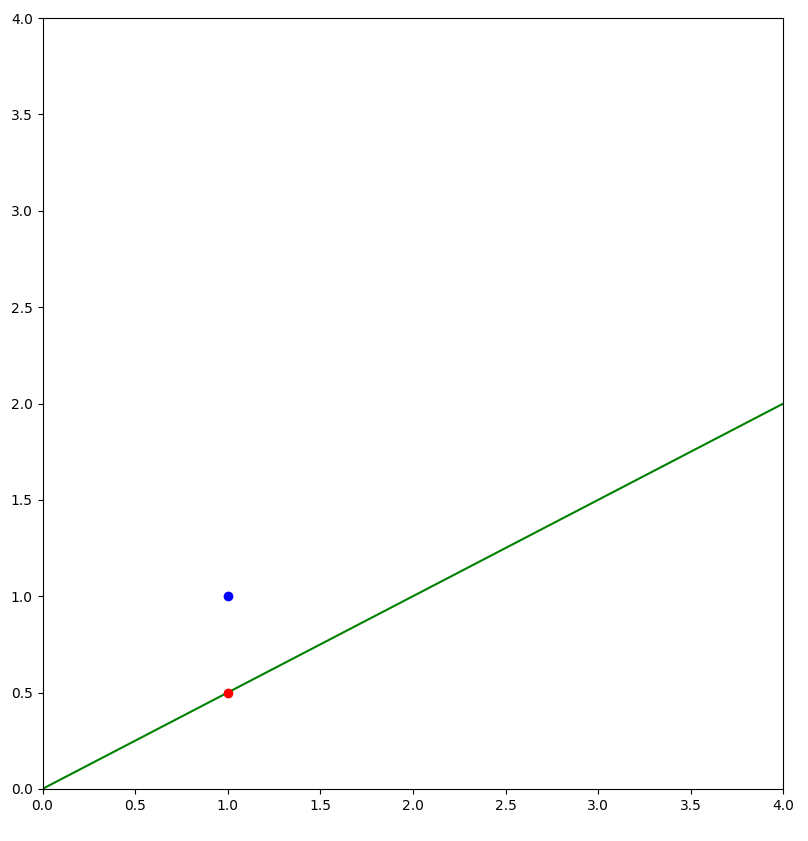
\includegraphics[width=0.8\linewidth]{Screenshots/task7_3.png}
    \end{figure}
    \bigbreak
    
    4. $\min_x \norm{x}_1 \: s.t. \norm{\Phi x - y}_{\infty} \le \epsilon$
    
    Пусть $s = [|x_1|, |x_2|, ..., |x_n|]$, $\epsilon_v$ - вектор состоящий из $\epsilon$, вектор переменных $[s; x]$. Тогда задачу оптимизации можно переписать как
    
    \begin{align*}
        \min 1^Ts\\
        s.t. \: x &\le s\\
        x &\ge -s\\
        \Phi x - y &\le \epsilon_v\\
        -\Phi x + y &\le \epsilon_v
    \end{align*}
    
    Выразми $c, A, b$:
    \begin{align*}
        c = \left[\begin{matrix} 1_v\\ 0_v \end{matrix} \right], \:
        A = \left[
            \begin{matrix}
                -I & I\\
                -I & -I \\
                0_m & \Phi \\
                0_m & -\Phi
            \end{matrix}
            \right], \:
        b = \left[
            \begin{matrix}
                0_v \\
                0_v\\
                \epsilon_v + y\\
                \epsilon_v - y
            \end{matrix}
            \right]
    \end{align*}
    
    \newpage
    Код решения:
    \lstinputlisting{Source/task7_4.py}
    
    Визуализация решения. Красная точка - $\Phi x_*$, синяя - $y$.
    \begin{figure}[H]
        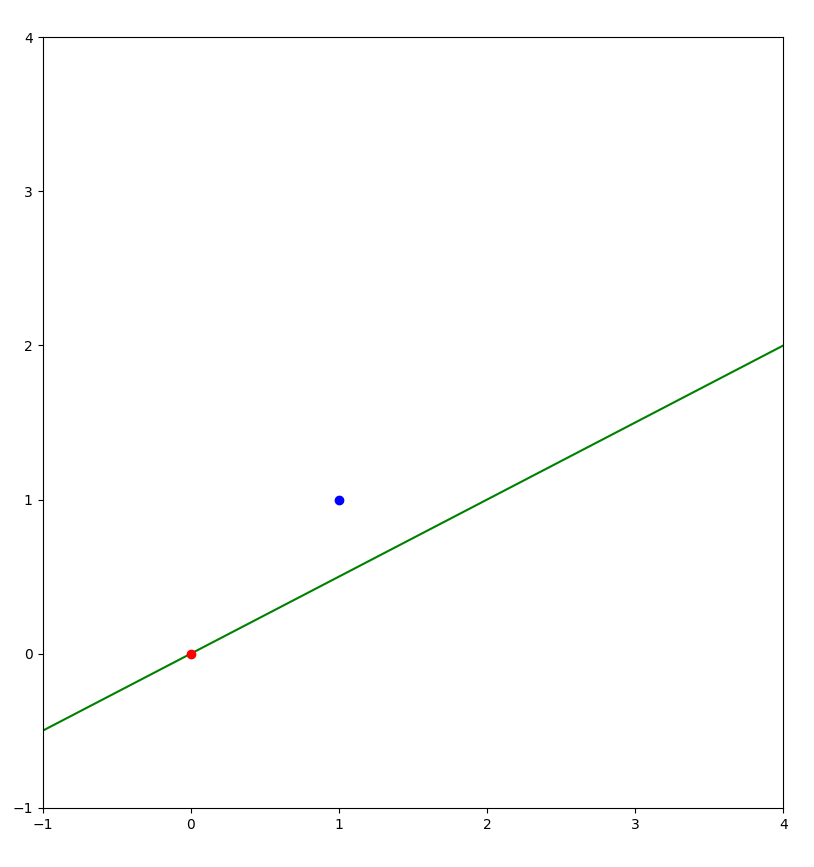
\includegraphics[width=0.8\linewidth]{Screenshots/task7_4.png}
    \end{figure}
    \bigbreak
    
    \bigbreak
    \subsection*{Задача 8}
    Найти $Z = \left[\begin{matrix} A & B \\ C & D \end{matrix} \right]$, 
    или $z = [A, B, C, D]^T = \vect(Z^T)$, если известны значения вертикальной и горизонтальной проекций (суммы элементов столбцов и строк, соответственно).  
    \begin{figure}[h!]
        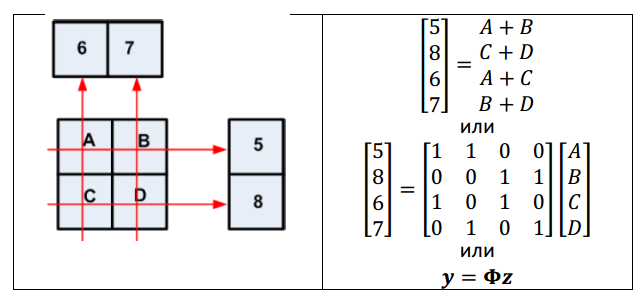
\includegraphics[width=0.8\linewidth]{Screenshots/scheme8.png}
    \end{figure}
    
    Существует бесконечне число векторов $z$, которые являются решениями данной системы уравнений. Пусть также известно, что $z$ имеет разреженное представление в базисе $\Psi$:
    \begin{align*}
        \Psi = \left[
            \begin{matrix}
                1 & 3 & 0 & 5\\
                2 & 0 & 2 & 1\\
                1 & 1 & 4 & 0\\
                0 & 2 & 3 & 2
            \end{matrix}
            \right],
    \end{align*}
    
    Найти $Z$ решая задачу оптимизации:
    \begin{align*}
        \min_x \norm{x}_p s.t. \Phi \Psi x = y
    \end{align*}
    для различных значений $p$.
    
    Матрица $\Phi$ имеет ранг равный 3, и 4 строки. Уберем из неё последнюю строку строку, являющуюся линейной комбинацей верхних трех, и не на что не влеющую.
    \bigbreak
    
    Инициализация:
    \lstinputlisting[firstline=1, lastline=20]{Source/task8.py}
    \newpage
    
    1. $p = 0$. Полным перебором для $k = 1, 2, ..., m $
    \bigbreak
    
    Будем перебирать комбинации столбцов, которые мы оставим и затем пробовать решить полученную систему методом наименьших квадратов. Если ошибка полученного решения мала ($ < 10^{-10} $), то решение найдено. Добавим его в массив решений и запомним, что для данного k (количества ненулевых столбцов) решение найдено и большие k рассматривать нет смысла.
    \lstinputlisting[firstline=24, lastline=46]{Source/task8.py}
    
    Найдено единственное решение для $k = 2$
    \begin{align*}
        x = \left[\begin{matrix} 1\\ 0\\ 1\\ 0 \end{matrix}\right], 
        z = \left[\begin{matrix} 1\\ 4\\ 5\\ 3 \end{matrix}\right]
    \end{align*}
    \newpage
    
    2. $p = 1$. Переформулировать как задачу линейного программирования и использовать функцию cvxopt.solvers.lp для получения решения.
    \bigbreak
    
    Задача оптимизации
    \begin{align*}
        \min_{x} \norm{x}_1\\
        s.t. \: Ax = y
    \end{align*}
    
    Пусть $s = [|x_1|, |x_2|, ..., |x_n|]^T$, вектор переменных $ [s; x] $, условия:
    \begin{align*}
        x &\le s\\
        x &\ge -s\\
        Ax &= y
    \end{align*}
    тогда решение методом линейного программирования выглядит следующим образом.
    
    \lstinputlisting[firstline=50, lastline=69]{Source/task8.py}
    
    Получен результат аналогичный результату в пункте 1.
    \newpage
    
    3. $p = 2$. Перейти к задаче оптимизации без ограничений используя представление $x = x_0 + Uw$, где $x_0$ - произвольное решение, а столбцы матрицы $U$ образуют базис $null(A)$.
    \bigbreak
    
    Решая недоопределенную систему $Ax = y$ получаем
    \begin{align*}
        x = Uw + x_0,\\ \text{где }
        U = \frac{1}{29}\left[\begin{matrix} 29\\ 19\\ -6\\ -22 \end{matrix}\right], 
        x_0 = \frac{1}{29}\left[\begin{matrix} 0\\ -19\\ 35\\ 22 \end{matrix}\right]
    \end{align*}
    
    Решим задачу оптимизации:
    \begin{align*}
        \min_w \norm{Uw + x_0}_2^2
    \end{align*}
    \begin{align*}
        d\norm{Uw + x_0}_2^2 &= d(Uw + x_0)^T(Uw + x_0) = 2(Uw + x_0)^TUdw\\
        U^T(Uw + x_0) &= 0\\
        w &= -\frac{U^Tx_0}{U^TU}\\
        x &= U\left(-\frac{U^Tx_0}{U^TU}\right) + x_0 = 
        \left(I - \frac{UU^T}{U^TU}\right)x_0
    \end{align*}
    
    Функция выпуклая, значит найденая стационарная точка будет глобальным минимумом.    
    
    \lstinputlisting[firstline=73, lastline=81]{Source/task8.py}
    
    Решение отличается от первых двух, но похоже на них.
\end{document}

    


    
    
